\chapter{Diagrams}
\begin{figure}[H]
    \begin{center}
        % original from idea
        %\scalebox{0.34}[0.475]{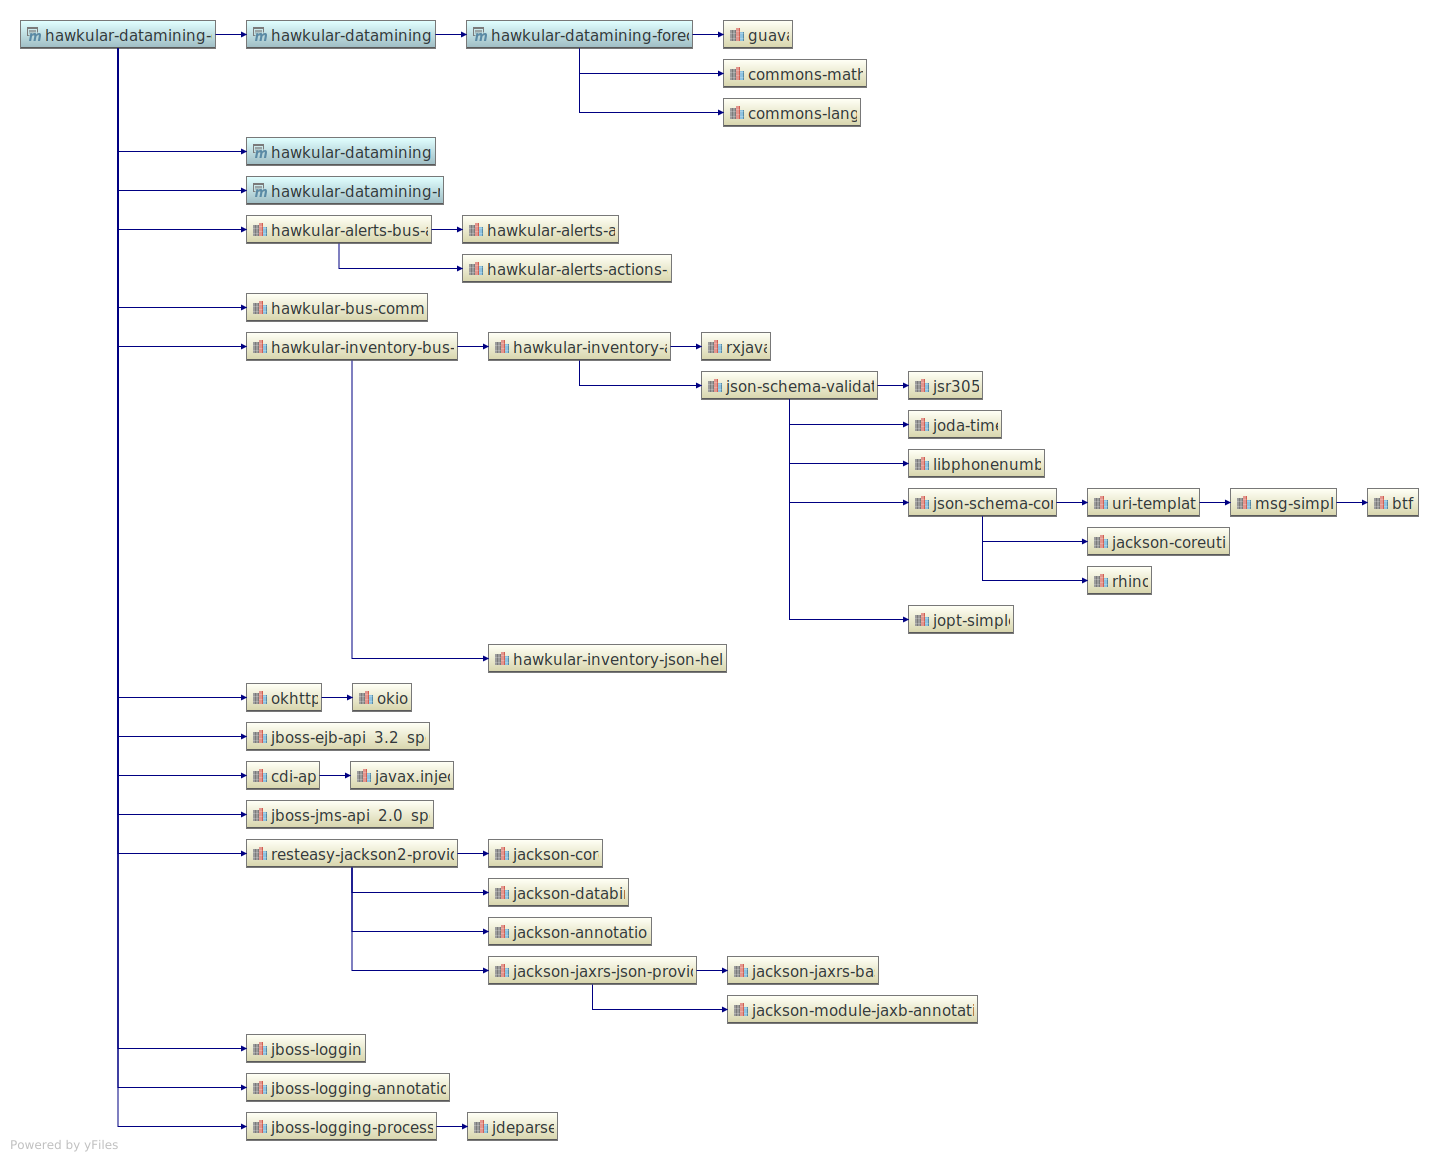
\includegraphics{img/src/maven-deps-tree.pdf}}
        \scalebox{0.6}{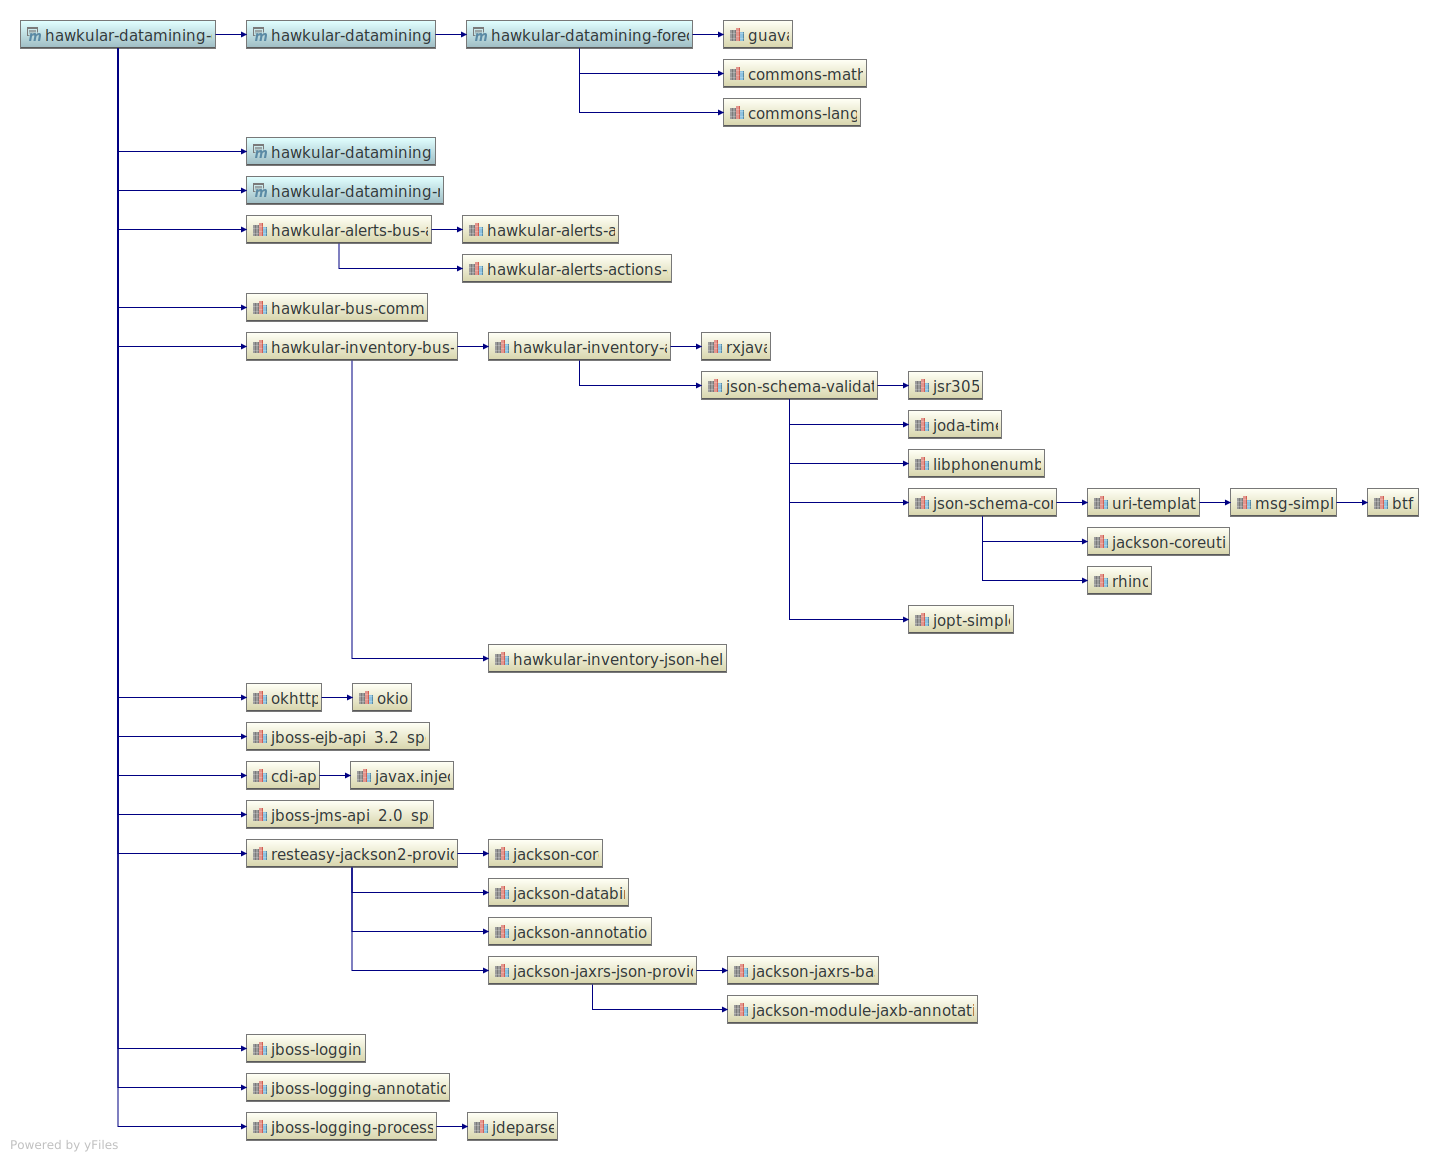
\includegraphics{img/src/maven-deps-tree.pdf}}
        \caption{Dependency tree of maven artifacts.}
        \label{appen:maven-deps}
    \end{center}
\end{figure}

\begin{figure}[H]
    \begin{center}
        \scalebox{0.35}[0.21]{\includegraphics[angle=90]{img/src/class-diagram.pdf}}
        \caption{Partial class diagram of \texttt{datamining-forecast} and \texttt{datamining-api}.}
        \label{appen:class-diagram}
    \end{center}
\end{figure}

\chapter{Predictive Charts}
\begin{figure}[H]
    \begin{center}
        \scalebox{0.6}[0.443]{\includegraphics[angle=90]{img/hawkular-simple.pdf}}
        \caption{Predictive chart for simple exponential smotohing.}
        \label{appen:hawkular-simple}
    \end{center}
\end{figure}
\begin{figure}[H]
    \begin{center}
        \scalebox{0.6}[0.5]{\includegraphics[angle=90]{img/hawkular-double.pdf}}
        \caption{Predictive chart for double exponential smotohing.}
        \label{appen:hawkular-double}
    \end{center}
\end{figure}
\begin{figure}[H]
    \begin{center}
        \scalebox{0.6}[0.5]{\includegraphics[angle=90]{img/hawkular-triple.pdf}}
        \caption{Predictive chart for triple exponential smotohing.}
        \label{appen:hawkular-triple}
    \end{center}
\end{figure}

\chapter{Content of the CD}
